\documentclass[tikz,border=6pt]{standalone}
\usepackage{pgfplots}
\pgfplotsset{compat=1.18}
\begin{document}
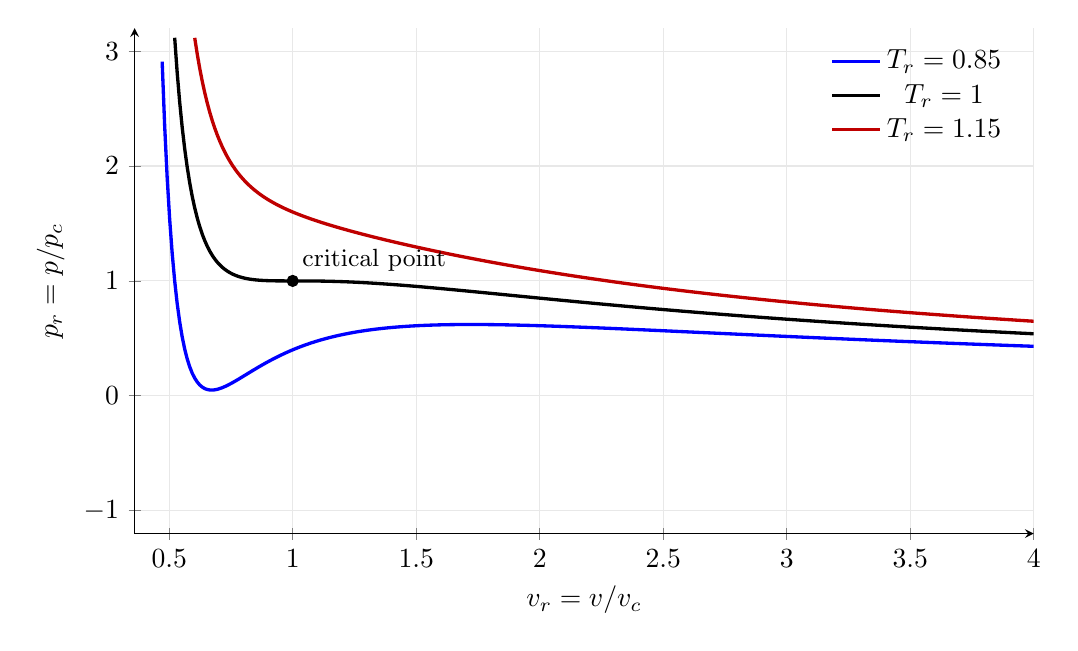
\begin{tikzpicture}
\begin{axis}[
 width=13cm,height=8cm,axis lines=left,
 xlabel={$v_r=v/v_c$},ylabel={$p_r=p/p_c$},
 xmin=.36,xmax=4,ymin=-1.2,ymax=3.2,
 samples=360,domain=.36:4,
 restrict y to domain=-1.2:3.2,
 unbounded coords=jump,
 legend style={draw=none,fill=none,at={(.98,.98)},anchor=north east},
 grid=major,grid style={gray!18}
]
% Reduced van der Waals equation: p_r=8 T_r/(3v_r-1)-3/v_r^2.
\addplot[very thick,blue] {8*0.85/(3*x-1)-3/x^2};
\addlegendentry{$T_r=0.85$}
\addplot[very thick,black] {8/(3*x-1)-3/x^2};
\addlegendentry{$T_r=1$}
\addplot[very thick,red!75!black] {8*1.15/(3*x-1)-3/x^2};
\addlegendentry{$T_r=1.15$}
\addplot[only marks,mark=*,mark size=2pt] coordinates {(1,1)};
\node[anchor=south west,font=\small] at (axis cs:1,1) {critical point};
\end{axis}
\end{tikzpicture}
\end{document}
